\section{Hagan Rowlenstino/1174040}
	\subsection{Pemahaman Teori}
	\begin{enumerate}
	\item format file csv dapat menyimpan data dalam jumlah yang sangat besar juga diperuntukkan untuk export dan import untuk spreadsheet ataupun database. Singkatan CSV pertamakali di pakai pada tahun 1983, dimana value yang dipisahkan dengan koma lebih mudah untuk diketik daripada data yang sejajar dengan kolom yang tetap. contohnya seperti gambar dibawah ini.

	\begin{figure}[ht]
            \centerline{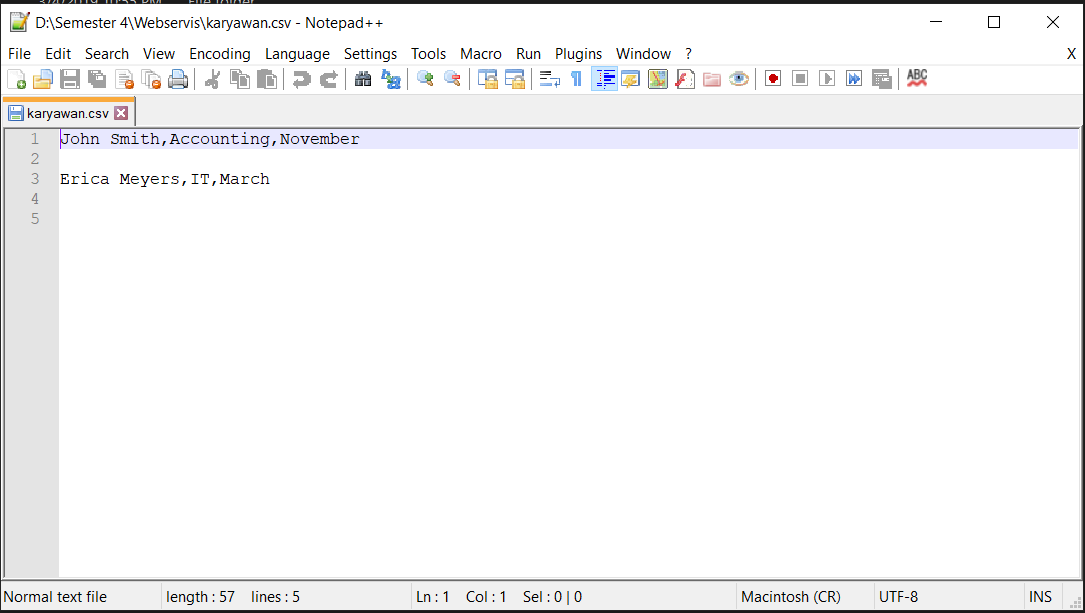
\includegraphics[width=0.5\textwidth]{figures/chapter4/1174040_csv.png}}
            \caption{Contoh CSV}
            \label{1174040_csv}
            \end{figure}

	\item Ms.Excel , NotePad, notepad++, sublime, dan texteditor lainnya

	\item caranya adalah :
		\begin{itemize}
			\item untuk write :
			\begin{enumerate}
				\item Download template csv
				\item Buka browser lalu menuju ke Google Sheet
				\item Tekan tombol merah di pojok kanan bawah
				\item Lalu pilih upload file untuk mengupload template yang sudah di download sebelumya
				\item Edit sesuai yang diinginkan
				\item Setelah selesai, lalukan eksport ke CSV dengan cara klik file lalu download as setelah itu pilih CSV
			\end{enumerate}
			\item untuk read :
			\begin{enumerate}
				\item buka Ms.Excel
				\item pilih Data lalu Get External Data dan pilih From Text
				\item lalu pilih file csv nya
				\item pilih Delimeted lalu Next
				\item checklist di box Tab dan Comma
				\item lalu klik finish
			\end{enumerate}
		\end{itemize}	
	\item Library CSV berisikan fungsi -fungsi dan kelas yang akan dipakai dalam pengerjaan file CSV

	\item Pandas diciptakan pada tahun 2008 oleh Wes McKinney dan diperbaharuin pada tahun 2010 oleh Sien Chang. yang fungsinya untuk melakukan analisa data seperti import dan export data.

	\item Fungsi - funsi library csv adalah :
		\begin{itemize}
			
			\item \begin{verbatim}csv.reader(csvfile, dialect='excel', **fmtparams)\end{verbatim} : digunakan untuk membaca line di csv
			\item \begin{verbatim}csv.writer(csvfile, dialect='excel', **fmtparams)\end{verbatim} : untuk menulis line di csv
			\item \begin{verbatim}csv.register_dialect(name[, dialect[, **fmtparams]]) \end{verbatim}: untuk asosiasikan dialect dengan name, dimana name harus string
			\item \begin{verbatim}csv.unregister_dialect(name)\end{verbatim} : menghapus dialect yang terasosiasi dengan name
			\item \begin{verbatim}csv.get_dialect(name)\end{verbatim} : mengnembalikan hasil dialect yang terasosisasi dengan name
			\item \begin{verbatim}csv.list_dialects() \end{verbatim}: menampilkan semua dialect yang ada
			\item \begin{verbatim}csv.field_size_limit([new_limit])\end{verbatim} : menamplikan field maksimal ayng di berikan oleh pembubat parse.

		\end{itemize}

	\item Pandas mengngunakan sistem dataframe yang memeprbolehkan kita untuk memasukkan sebuah file ke dalam tabel vitual seperti spreadsheet.kita dapat mengolah dengan fungsi - fungsi  seperti join, distinct, group by, agregasi dan funsi lain seperti dalam SQL tetapi dibuat pada tabel yang dimuat di file ke ram
	\end{enumerate}

\section{IrvanRizkiansyah/1174043}
	\subsection{Pemahaman Teori}
		\begin{enumerate}
			\item \begin{itemize}
					\item Fungsi : File csv berfungsi untuk pencarian data akan menjadi lebih mudah dan cepat, dan juga mempermudah penginputan data ke dalam database secara sederhana.
					\item Sejarah : File csv muncul pertama kali sekitar 10 tahun sebelum Personal Computer (PC) pertama  didunia yaitu sejak sekitar tahun 1972, akan tetapi sebutan file csv digunakan pertama kali pada tahun 1983.
					\item Contoh : 
						\begin{figure} [ht]
							\centerline{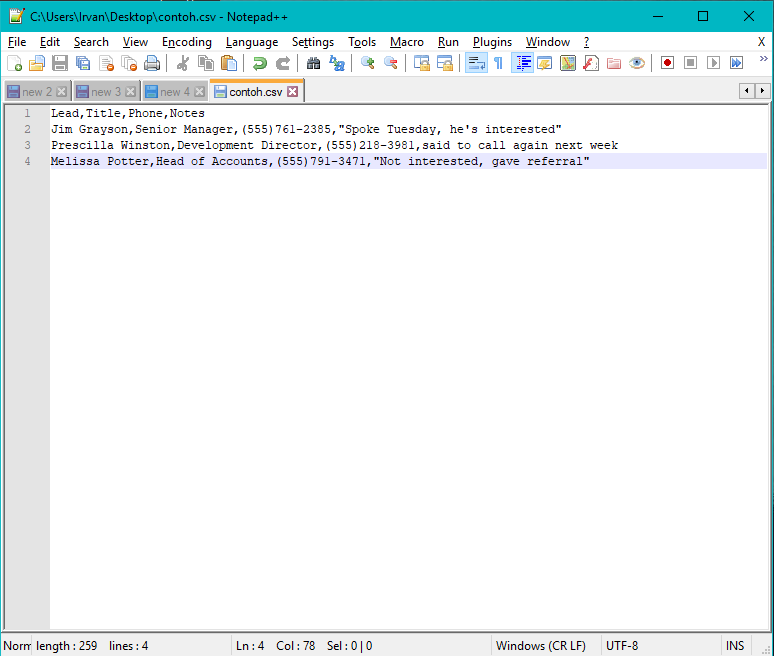
\includegraphics[width=0.6\textwidth]{figures/chapter4/Contoh_CSV.png}}
							\caption{Contoh CSV}
							\label{Contoh CSV}
						\end{figure}

					\ref{Contoh_CSV}
				\end{itemize}
			
			\item Ada banyak aplikasi yang dapat membuat file berformat CSV, diantaranya adalah :
				\begin{itemize}
					\item Notepad
					\item Notepad++
					\item Microsoft Excel
					\item Corel Quatro Pro
					\item Apache Open Office, dan masih banyak yang lainnya.
				\end{itemize}
			
			\item Cara menulis file csv menggunakan Excel :
				\begin{enumerate}
					\item Buka aplikasi Microsoft Excel kemudian buat dokumen baru
					\item Tulis judul kolom untuk setiap informasi yang ingin di rekam atau catat, kemudian tulis informasi - informasi dalam kolom dengan sesuai.
					\item Jika sudah selesai maka save dengan cara pilih menubar File lalu pilih Save As
					\item Lalu isikan nama file tersebut dan rubah dengan memilih format file yang tersedia tersebut menjadi .csv
					\item File csv sudah berhasil terbuat menggunakan Microsoft Excel
				\end{enumerate}
			\item Cara membaca file csv menggunakan Excel :
				\begin{enumerate}
					\item Buka aplikasi Microsoft Excel kemudian pilih menu Open
					\item Cari tempat file csv yang ingin dibuka, kemudian pilih Open
					\item File csv sudah berhasil dibaca menggunakan Microsoft Excel
				\end{enumerate}
			
			\item Pada file csv, tanda baca koma diartikan sebagai pembatas suatu kolom. List-directed input output didefinisikan dalam FORTRAN 77. List-directed input menggunakan tanda baca koma atau spasi sebagi pembatas, sehinnga karakter yang tidak dikutip tidak dapat mengandung tanda baca koma ataupun spasi. Hal tersebut yang diadopsi oleh file csv. format csv didukung dengan library untuk banyak bahasa pemrograman, kebanyakan yang menspesifikasikan pembatas field, pemisah desimal, pengkodean karakter, dan yang lainnya.
			
			\item Pada tahun 2008, pengembangan pandas dimulai oleh AQR Capital Management. Pada akhir tahun 2009 pandas menjadi Open Sourced, dimana disupport oleh banyak komunitas atau individu di dunia untuk mengembangkan pandas. Sejak tahun 2015, pandas menjadi NumFOCUS proyek sponsor, ini juga membantu suksesnya pengembangan dari pandas itu sendiri. pandas merupakan struktur data dan data analysis tools untuk bahasa pemrograman Python, dan merupakan BSD-licensed library yang menjadikannya memiliki performa yang tinggi.
			
			\item 
				\begin {itemize} 
					\item Tanda baca koma : Menjadi pemisah antar kolom
					\item Tanda baca kutip dua : Menjadi cara untuk memasukan sebuah kalimat atau untuk memasukan karakter spasi sebagai data pada kolom informasi
					\item Inputan pada baris pertama akan menjadi Header, dimana akan menjadi nama sebuah kolom, dan masih banyak yang lainnya
				\end{itemize}
			
			\item Pada pandas sedikit berbeda, dimana inputan data berbentuk seperti peng-inputan pada variabel pada umumnya, hanya saja menggunakan tanda kutip satu untuk menandakan sebuah informasi pada kolom kemudian tanda kurung kotak yang didalamnya berisi informasi data dari kolom tersebut. dan lain sebagainya.
			
		\end{enumerate}

\subsection{Luthfi Muhammad Nabil/1174035}
\subsubsection{Fungsi, Sejarah, dan Contoh file CSV}
\begin{itemize}
	\item Fungsi \linebreak File CSV (Comma Separated Values) adalah tipe file khusus yang menyimpan informasi dengan metode dipisahkan dengan koma. File CSV berfungsi untuk menjadi perantara untuk beberapa aplikasi yang memiliki basis data saat mengirim data. CSV dapat dibuka di berbagai text editor
	yang ada. Dengan bentuk filenya yang dinamis memungkinkan file CSV dapat dimanipulasi dan dapat menyimpan informasi dengan skala besar.
	\item Sejarah \linebreak CSV sudah digunakan sejak tahun 1972 yang dapat dikompilasi pada bahasa pemrograman IBM Fortran. Saat itu, data yang dipisahkan oleh koma jika isinya memiliki spasi maka harus diberi tanda petik di awal dan akhir isi dari data tersebut. Nama CSV baru mulai digunakan pada tahun 1983. Pada panduan dari Osborne Executive Computer mendokumentasikan kutipan yang membolehkan isi karakter memiliki koma.  Pada tahun 2005 dengan RFC4180, CSV didefinisikan sebagai MIME Content Type. lalu pada tahun 2013, defisiensi dari RFC4180 dipecahkan oleh rekomendasi dari W3C. Pada tahun 2014, IETF mempublikasi RFC7111 yang mendeskripsikan pecahan Uniform Resource Identifier(URI) ke dokumen CSV. RFC7111 menjelaskan bagaimana baris, kolom dapat dipilih dalam dokumen CSV menggunakan indeks posisi. Pada Tahun 2015, W3C mempublikasikan draft rekomendasi untuk CSV-metadata standards yang dimulai dengan rekomendasi pada bulan Desember dengan tahun yang sama. 
	\item Contoh File CSV \begin{itemize}
							\item 
							CSV pada Excel \ref{1174035_CSVExcel}
							\begin{figure}[!htbp]
								\centering
								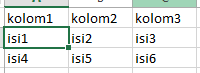
\includegraphics[height=4cm, width=7cm]{figures/chapter4/1174035_CSVExcel.jpg}
								\caption{Contoh CSV Pada Excel}
								\label{1174035_CSVExcel}
							\end{figure}
							\item \begin{figure}[!htbp]
								\centering
								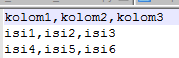
\includegraphics[height=4cm, width=7cm]{figures/chapter4/1174035_CSVText.jpg}
								\caption{Contoh CSV Pada Text}
								\label{1174035_CSVText}
							\end{figure}
							CSV pada Text Editor \ref{1174035_CSVText}
							
						  \end{itemize}
\end{itemize}
\subsubsection{Aplikasi Yang dapat membuat file CSV}
Berikut file yang dapat membuat file CSV
\begin{itemize}
	\item Spreadsheet \linebreak Spreadsheet merupakan aplikasi yang dapat membuat CSV hanya dengan memasukan data sesuai baris dan kolom yang diinginkan. Contoh spreadsheet seperti Google Spreadsheet, Microsoft Excel, dan aplikasi lainnya. 
	\item Bahasa Pemrograman \linebreak Bahasa pemrograman merupakan media yang dapat untuk membuat aplikasi yang dapat membuat file CSV khusus untuk bahasa pemrograman yang support dengan pembuatan file CSV. Seperti Python, C Sharp, dan lain sebagainya.
	\item Text Editor \linebreak Text editor juga dapat membuat file CSV, untuk membuat dengan Text Editor cukup dengan membuat file sesuai format CSV dan save file tersebut dengan ekstensi .CSV.
\end{itemize}
\subsubsection{Menulis dan Membaca file CSV}
Berikut cara menulis dan membaca file CSV : 
\begin{itemize}
	\item Menulis : \begin{enumerate}
						\item Buka file CSV dengan spreadsheet
						\item Klik Cell yang mau diisi
						\item Masukan data yang mau diisi pada cell tersebut
						\item Lalu save file dengan format .CSV
					\end{enumerate}
	\item Membaca : \begin{enumerate}
						\item Buka file CSV dengan spreadsheet						
					\end{enumerate}
\end{itemize}
\subsubsection{Sejarah Library CSV Python}
Library CSV pada python merupakan library yang paling umum untuk import export data pada spreadsheet dan basis data dengan format sesuai dengan standarisasi RFC4180. Seiring dengan lahirnya bahasa pemrograman python, library mulai dibuat dan dikembangkan sampai akhirnya pada tahun 2003, pembuatnya Kevin Altis dan lainnya telah merilis versi final untuk library Python CSV. 
\subsubsection{Sejarah Library Pandas Python}
Pandas (Python Data Analysis Library) adalah library open source yang digunakan untuk melakukan data manajemen dan data analysis. Pandas diciptakan pada tahun 2008 oleh Wes McKinney dan diperbaharui oleh Sien Chang pada tahun 2010. Inspirasi dari pembuatan pandas muncul pada komunitas yang membutuhkan library khusus untuk analisis data. 
\subsubsection{Fungsi - fungsi yang terdapat di library CSV}
\begin{itemize}
	\item \begin{verbatim} csv.reader(csvfile, dialect='excel', **fmtparams) \end{verbatim} Untuk mengembalikan	object reader yang akan mengambil setiap line pada csv yang diambil. Data setiap baris diambil saat next() dipanggil. Berikut contohnya : \lstinputlisting[firstline=1, lastline=6]{src/chapter4/chap4_1174035_teori.py}
	\item \begin{verbatim} csv.writer(csvfile, dialect='excel', **fmtparams) \end{verbatim} Mengembalikan file pembuat object untuk dapat mengkonversi data pada python ke file CSV yang akan dibuat. Berikut contoh penggunaan csv.writer : \lstinputlisting[firstline=8, lastline=14]{src/chapter4/chap4_1174035_teori.py}
	\item \begin{verbatim} csv.register_dialect(name[, dialect[, **fmtparams]]) \end{verbatim} Mengasosiasikan dialek dengan nama, nama yang dimasukkan harus berupa karakter.
	\item \begin{verbatim} csv.unregister_dialect(name) \end{verbatim}
	Menghapus asosiasi dialek dengan nama pada registry dialek.
	\item \begin{verbatim} csv.get_dialect(name) \end{verbatim}
	Mengambil dialek yang telah diasosiasikan dengan nama. 
	\item \begin{verbatim}  csv.list_dialects() \end{verbatim} Mengembalikan dialek yang telah diregistrasi.
	\item \begin{verbatim} csv.field_size_limit([new_limit]) \end{verbatim} Mengembalikan maksimal kolom data yang diperbolehkan oleh pembaca.
\end{itemize}
\subsubsection{Fungsi - fungsi yang terdapat di library Pandas}
\begin{itemize}
	\item \begin{verbatim} pandas.read_csv(filepath_or_buffer[, sep, …]) \end{verbatim} Untuk membaca file CSV dan menyimpannya ke DataFrame
	\item \begin{verbatim} pandas.read_excel(io[, sheet_name, header, names, …])  \end{verbatim} Membaca file excel dan menyimpannya ke DataFrame
	\item \begin{verbatim} to_csv([path, index, sep, na_rep, …]) \end{verbatim}
	Untuk membuat file CSV dari data yang ada	
\end{itemize}

\section{Faisal Najib Abdullah}
\subsection{Pemahaman Teori}
\begin{enumerate}
    \item Apa itu fungsi file csv, jelaskan sejarah dan contoh ?
    \par
    File CSV Nilai Berbatas Koma adalah tipe file khusus yang dapat Anda buat atau edit di Excel. File CSV menyimpan informasi yang dipisahkan oleh koma, bukan menyimpan informasi dalam kolom. Saat teks dan angka disimpan dalam file CSV, mudah untuk memindahkannya dari satu program ke program lain.
    \par 
	File CSV dibuat oleh program yang menangani sejumlah data yang besar. CSV merupakan cara yang nyaman untuk mengekspor data dari spreadsheet dan basis data serta mengimpor atau menggunakannya dalam program lain. Misalnya, Anda dapat mengekspor hasil program penambangan data ke file CSV dan kemudian mengimpornya ke dalam spreadsheet untuk menganalisis data, menghasilkan grafik untuk presentasi, atau menyiapkan laporan untuk publikasi.
    \par
	Contohnya, Anda dapat mengekspor kontak dari Google ke dalam file CSV, kemudian mengimpornya ke Outlook.
    
    \item Aplikasi-aplikasi apa saja yang bisa menciptakan file csv?
    Pada Windows
    \begin{itemize}
        \item Microsoft Excel 2013
        \item Microsoft Works
        \item CCorel Quattro Pro
        \item Apache OpenOffice
        \item LibreOffice
        \item Microsoft Notepad
        \item Intuit Quicken 2015
        \item GenScriber
    \end{itemize}
    Pada Mac OS
    \begin{itemize}
        \item Microsoft Excel 2011
        \item Planamesa NeoOffice
        \item Apache OpenOffice
        \item LibreOffice
        \item GenScriber
    \end{itemize}
    Pada Linux
    \begin{itemize}
        \item Apache OpenOffice
        \item LibreOffice
        \item GenScriber
    \end{itemize}
    
    \item Jelaskan bagaimana cara menulis dan membaca file csv di excel atau spreadsheet?
	\begin{itemize}
        \item Cara menulis file csv harus berupa baris dan kolom atau bisa juga di sebut berupa tabel.
        \item Untuk membacanya file csv dipisahkannya menggunakan koma atau titik koma.
    \end{itemize}
    
    \item Jelaskan sejarah library csv?
	Library csv menyediakan fungsionalitas untuk membaca dan menulis ke file CSV. Dirancang untuk bekerja di luar kotak dengan file CSV yang dihasilkan Excel, memudahkan untuk bekerja dengan berbagai format CSV. Library csv berisi objek dan kode lain untuk membaca, menulis, dan memproses data ke file CSV.
    
    \item Jelaskan sejarah library pandas?
	panda adalah pustaka Python open-source yang menyediakan alat analisis data kinerja tinggi dan struktur data yang mudah digunakan. panda tersedia untuk semua instalasi Python, tetapi itu adalah bagian penting dari distribusi Anaconda dan bekerja sangat baik di notebook Jupyter untuk berbagi data, kode, hasil analisis, visualisasi, dan teks naratif.

    \item Jelaskan fungsi-fungsi yang terdapat di library csv?
	Terdapat 2 fungsi yang bisa digunakan oleh library csv
    Pertama,fungsi membaca file csv.
    fungsi ini bisa menggunakan list dan dictionary
    Dengan list :
    \lstinputlisting[firstline=11, lastline=21]{src/chapter4/1174042_csv.py}
    Dengan dictionary :
    \lstinputlisting[firstline=24, lastline=33]{src/chapter4/1174042_csv.py}
    Kedua,fungsi menulis file csv.
    \lstinputlisting[firstline=36, lastline=40]{src/chapter4/1174042_csv.py}
    
    \item Jelaskan fungsi-fungsi yang terdapat di library pandas
	Hampir sama dengan library csv,tp library pandas penulisannya lebih sederhana dan terlihat lebih rapih dari pada library csv.
    \lstinputlisting[firstline=43, lastline=44]{src/chapter4/1174042_csv.py}
    

\end{enumerate}

\section{Fathi Rabbani / 1164074}
\subsection{Teori}
\begin{enumerate}
\item Sejarah dan Penjelasan CSV
\subitem Penggunaan dari format file CSV itu sendiri untuk memudahkan pembuatan data dengan menggunakan tanda koma sebagai pembatas dari datanya agar mudah untuk dibaca pada kolom.
\subitem CSV sendiri dibuat untuk dapat menangani pembuatan sejumlah data yang berukuran besar, mempermudah program dalam membaca datanya kedalam kolom - kolom. seperti contoh dalam membacanya menggunakan aplikasi Excel sehingga mempermudah dalam proses import dan eksport datanya. csv sendiri sudah ada pada tahun 1972 dengan pengembangnya adalah IBM namun penggunaannya masuk pada tahun 1983 yang berbarengan dengan adanya SuperCalc spreadsheet.

\item Aplikasi CSV
\begin{itemize}
\item Microsoft Excel
\item Open Office Calc
\item Google Docs
\item Libre Office
\item Apache Open Office
\end{itemize}

\item Menulis dan Membaca csv di Excel atau Spreadsheet
\subitem Menulis, cara menuliskan csv adalah dengan menggunakan tanda baca koma pada bagian data yang ingin dipisah contohnya \lstinputlisting[firstline=8, lastline=29]{src/chapter4/coba.csv}
\subitem Membaca, file csv dapat dibaca pada program aplikasi Excel dengan menampilkan hasil data dari setiap data yang dipisah dengan tanda baca koma menjadi kolom - kolom hasilnya ada pada \ref{fig1}

\item Library CSV
\subitem CSV atau comma separated value adalah salah satu tipe file yang digunakan secara luas di dunia programming. Tidak hanya itu CSV pun sering digunakan dalam pengolahan informasi yang dihasilkan spreadsheet untuk diproses lebih lanjut melalui mesin analitik. CSV pun dianggap sebagai file yang agnostik karena dapat digunakan oleh berbagai database untuk proses backup data.

\item Library Pandas
\subitem pandas merupakan library pada pemrograman python yang berguna untuk mengolah dan meyediakan struktur data serta analisa data yang mudah untuk dibaca dan dipahami seperti pada struktur data tabel. pandas dapat melakukan proses perbandingan data, penggabungan dataset, penanganan dataset yang hilang dll. pandas dapat juga digunakan sebagai pemrosesan data Statistik dengan pembacaan datanya menggunakan struktur Spreadsheet.

\item Fungsi pada Library CSV
\begin{itemize}
\item Menulis data CSV
\lstinputlisting[firstline=8, lastline=29]{src/chapter4/coba.csv}
\item Hasil dari menullis data CSV
\lstinputlisting[firstline=31, lastline=37]{src/chapter4/coba.csv}
\item Membaca data CSV
\lstinputlisting[firstline=40, lastline=52]{src/chapter4/coba.csv}
\item Hasil pembacaan data CSV
\lstinputlisting[firstline=54, lastline=60]{src/chapter4/coba.csv}
\end{itemize}

\item Fungsi pada Library Pandas
\begin{itemize}
\item Kode
\lstinputlisting[firstline=62, lastline=67]{src/chapter4/coba.csv}
\item Hasil
\lstinputlisting[firstline=69, lastline=73]{src/chapter4/coba.csv}
\end{itemize}
\end{enumerate}

\begin{figure}[!htbp]
	\centering
	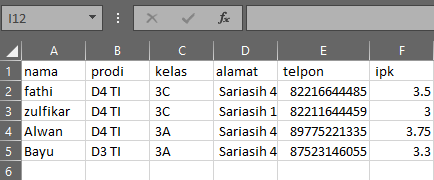
\includegraphics[width=1\textwidth]{figures/chapter4/1164074/1}
	\caption{hasil csv pada Excel}
	\label{fig1}
\end{figure}

\section {Kevin Natanael Nainggolan 1174059}
	\begin {enumerate}
		\item Apa itu fungsi csv, jelaskan sejarah dan contohnya 
			\lstinputlisting [firstline=10, lastline=14]{src/teoric4.py}
		\item Aplikasi-aplikasi apa saja yang bisa menciptakan file csv? 
			\lstinputlisting [firstline=18, lastline=22]{src/teoric4.py}
		\item Jelaskan bagaimana cara menulis dan membaca file csv di excel atau spreadsheet
			\lstinputlisting [firstline=26, lastline=39]{src/teoric4.py}
		\item Jelaskan sejarah library csv
			\lstinputlisting [firstline=43, lastline=50]{src/teoric4.py}
		\item Jelaskan sejarah library pandas
			\lstinputlisting [firstline=54, lastline=60]{src/teoric4.py}
		\item Jelaskan fungsi-fungsi yang terdapat di library csv
			\lstinputlisting [firstline=64, lastline=68]{src/teoric4.py}
		\item Jelaskan fungsi-fungsi yang terdapat di library pandas
			\lstinputlisting [firstline=72, lastline=75]{src/teoric4.py}
	\end {enumerate}

\section{Yusniar Nur Syarif Sidiq/1164089}
\subsection{Pemahaman Teori}

\begin{enumerate}

\item Apa itu fungsi file csv, jelaskan sejarah dan contoh.
	\subitem File csv merupakan jenis file khusus yang dapat kita buat dan edit di dalam Excel. File csv akan menyimpan informasi data yang dipisahkan dengan koma atau tanda titik koma, dimana artinya file csv tidak menyimpan data dalam bentuk kolom. Saat pertama kali rilis, excel menggunakan format file dalam bentuk biner yaitu BIFF sebagai format file utama. Namun setelah Microsoft merilis Ofice System 2007, Excel telah menggantikan format utamanya menjadi XML. Meskipun mendukung format XML baru, Excel masih mendukung format BIFF, tidak hanya itu excel juga telah mendukung format CSV, DBF, SYLK, DIF, dan format-format lainnya. Fungsi dari file csv itu sendiri adalah mempermudah dalam pencarian data dan pengimputan data ke dalam database sederhana. File csv mulai digunakan pada tahun 1983 akan tetapi format file csv sudah ada dari tahun 1972. Contoh file dengan format csv dapat dilihat pada figure \ref{YNCSV1}

	\begin{figure}[ht]
		\centering{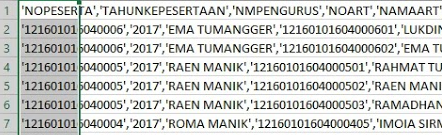
\includegraphics[scale=0.5]{figures/chapter4/YN/Chapter4/YNCSV1.png}}
		\caption{Contoh File CSV}
		\label{YNCSV1}
	\end{figure}

\item Aplikasi - aplikasi apa saja yang bisa menciptakan file csv.
	\subitem Untuk membuat file dengan format CSV, kita dapat menggunakan software bawaan Microfsoft Ofice yaitu Excel. Bukan hanya Microsoft Excel, kita juga dapat membuat file CSV dengan bantuan text editor. Jika kita ingin membuat file csv secara online dapat menggunakan Google Spreadshare. Apabila OS PC kita menggunakan Linux dapat menggunakan LibreOfficecalc.

\item Jelaskan bagaimana cara menulis dan membaca file csv di excel atau spreadsheet.
	\subitem Cara membuat file CSV dengan Excel
			\begin{itemize}
				\item Buka software Microsoft Excel
				\item Pilih new document
				\item Buatlah judul kolom yang ingin kita rekam
				\item Isikan informasi - informasi pada setiap kolom
				\item Simpan dengan menggunakan metode save as
				\item Cari dan pilih format csv
				\item Pilih button save untuk melakukan penyimpanan
			\end{itemize}
	\subitem Cara membaca file CSV dengan Excel
			\begin{itemize}
				\item Buka software Microsoft Excel
				\item Lakukan perintah open file
				\item Cari file csv yang sudah kita buat sebelumnya
				\item Pilih button open untuk membaca file csv pada Microsoft Excel
			\end{itemize}
	\subitem Cara membaca file csv dari Excel
		\lstinputlisting[firstline=1, lastline=9]{src/chapter4/1164089.py}
	\subitem Cara membuat file csv
		\lstinputlisting[firstline=12, lastline=16]{src/chapter4/1164089.py}

\item Jelaskan sejarah library csv. 
	\subitem Pada tahun 1972 adalah terbentuknya format file csv namun bukan hanya itu saja, pada saat itupun terbentuk juga yang namanya library pandas.Seiring dengan lahirnya bahasa pemrograman python, library mulai dibuat dan dikembangkan oleh Kevin Altis. Dengan kata lain CSV dibentuk pada tahun 1972 dan sudah satu paket baik dalam librarynya maupun format filenya. 

\item Jelaskan sejarah library pandas.
	\subitem Developer yang bernama Wes McKinney telah mengajarkan pandas pada tahun 2008 ketika ia berada di AQR Capital Management, karena kebutuhan akan alat kinerja tinggi yang fleksibel untuk melakukan analisis kuantitatif pada data keuangan. Sebelum meninggalkan AQR, dia dapat meyakinkan manajemen untuk mengizinkan membuka sumber library. Pegawai AQR lainnya yaitu Chang She, telah bergabung dengan upaya ini pada 2012 sebagai kontributor utama kedua ke library. Pada tahun 2015, pandas telah menandatangani sebagai proyek NumFocus yang disponsori secara fiskal. Pada saat itulah Library Pandas mulai berjalan dan digunakan.

\item Jelaskan fungsi-fungsi yang terdapat di library csv.
	\subitem Ada dua fungsi pada library csv, yaitu csv.reade dan csv.writer. Dimana fungsi tersebut memiliki tugas yang berbeda-beda. Untuk csv.reader bertugas sebagai membaca file csv sedangkan csv.writer bertugas membuat file csv.

\item Jelaskan fungsi-fungsi yang terdapat di library pandas.
	\subitem Untuk library pandas sama saja dengan library csv namun bedanya hanya cara penulisan source codenya saja. Untuk membaca file csv pada library pandas membutuhkan perintah pandas.read\_csv sedangkan untuk membuat file csv membutuhkan perintah pandas.write\_csv.

\end{enumerate}

\section{Dika Sukma Pradana 1174050}

\subsection{Pemahaman Teori}
\begin{enumerate}
	\item Definisi, Sejarah, dan Contoh
		\begin{itemize}
			\item Definisi
				\par Dalam komputasi, file CSV (Comma-separated values) adalah file teks terbatas yang menggunakan koma untuk memisahkan nilai. File CSV menyimpan data tabular (angka dan teks) dalam teks biasa. Setiap baris file adalah catatan data. Setiap catatan terdiri dari satu atau lebih bidang, dipisahkan dengan koma. Penggunaan koma sebagai pemisah bidang adalah sumber nama untuk format file ini.
			\item Sejarah 
				\par Nama Comma-separated values dan singkatan CSV digunakan pada tahun 1983. Manual untuk komputer Osborne Executive, yang membundel spreadsheet SuperCalc, mendokumentasikan konvensi kutipan CSV yang memungkinkan string mengandung koma yang disematkan, tetapi manual tersebut tidak menentukan konvensi untuk menanamkan tanda kutip dalam string yang dikutip.
				\par Daftar nilai yang dipisahkan dengan koma lebih mudah untuk diketik (misalnya ke dalam kartu berlubang) daripada data yang selaras dengan kolom tetap, dan cenderung menghasilkan hasil yang salah jika suatu nilai ditinju satu kolom dari lokasi yang dituju.
				\par File yang dipisahkan koma digunakan untuk pertukaran informasi basis data antara mesin dari dua arsitektur yang berbeda. Karakter teks-polos dari file CSV sebagian besar menghindari ketidakcocokan seperti urutan byte dan ukuran kata. File-file ini sebagian besar dapat dibaca oleh manusia, sehingga lebih mudah untuk mengatasinya tanpa adanya dokumentasi atau komunikasi yang sempurna.
				\par Inisiatif standardisasi utama - mentransformasikan definisi fuzzy de facto menjadi definisi yang lebih tepat dan de jure - adalah pada tahun 2005, dengan RFC4180, mendefinisikan CSV sebagai Tipe Konten MIME. Kemudian, pada 2013, beberapa kekurangan RFC4180 ditangani oleh rekomendasi W3C.
				\par Pada 2014 IETF menerbitkan RFC7111 yang menjelaskan aplikasi fragmen URI pada dokumen CSV. RFC7111 menentukan bagaimana rentang baris, kolom, dan sel dapat dipilih dari dokumen CSV menggunakan indeks posisi.
				\par Pada 2015 W3C, dalam upaya untuk meningkatkan CSV dengan semantik formal, mempublikasikan rancangan rekomendasi pertama untuk standar metadata CSV, yang dimulai sebagai rekomendasi pada bulan Desember tahun yang sama.
	
			\item Contoh 
				\begin{figure} [ht]
					\centerline{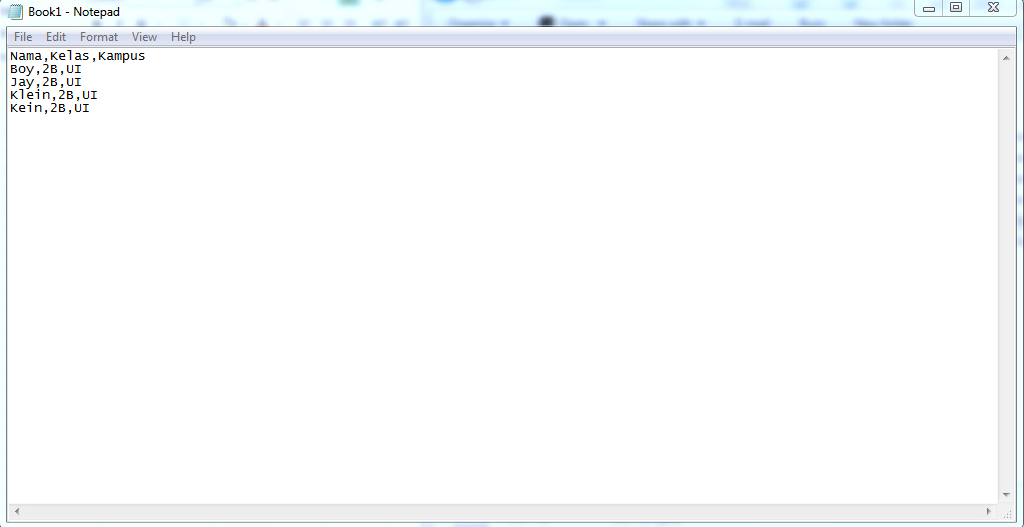
\includegraphics[width=0.6\textwidth]{figures/chapter4/csvd1ka.png}}
						\caption{Contoh CSV}
							\label{Contoh CSV}
				\end{figure}
			\ref{csvd1ka}
		\end{itemize}
		
		
	
	
	\item Ada banyak aplikasi yang dapat membuat file berformat CSV, diantaranya adalah :
				\begin{itemize}
					\item Microsoft Excel
					\item Corel Quatro Pro
					\item Apache Open Office
					\item CSVed
					\item CSVstar
					\item CSVpad
					\item Dan masih banyak lagi.
				\end{itemize}
		\item Cara menulis dan membaca file csv di excel		
	\begin{itemize}
	\item Cara menulis file CSV di Excel :
				\begin{enumerate}
					\item Buat dokumen baru di Excel
					\item Tambahkan judul kolom untuk setiap potongan informasi yang ingin dicatat
					\item Pilih File
					\item Save As
					\item Gunakan kotak menurun untuk memilih format CSV 
					\item Beri nama pada file
					\item Simpan
				\end{enumerate}
	\item Cara membaca file csv menggunakan Excel :
				\begin{enumerate}
					\item Buka aplikasi Microsoft Excel kemudian pilih menu Open
					\item Cari tempat file csv yang ingin dibuka 
					\item Kemudian pilih Open
					\item File csv sudah berhasil dibaca menggunakan Microsoft Excel
				\end{enumerate}
	\end{itemize}
	\item Sejarah library csv
		\par Nilai yang dipisahkan oleh koma adalah format data yang memberi tanggal lebih awal pada komputer pribadi lebih dari satu dekade: kompiler IBM Fortran di bawah OS atau 360 mendukungnya pada tahun 1972. Input atau output daftar-diarahkan didefinisikan dalam FORTRAN 77, disetujui pada tahun 1978. Input yang diarahkan daftar menggunakan koma atau spasi untuk pembatas, sehingga string karakter yang tidak dikutip tidak dapat mengandung koma atau spasi.
		
	\item Sejarah library pandas
		\par Pengembang Wes McKinney mulai mengerjakan panda pada 2008 ketika di AQR Capital Management karena kebutuhan akan alat kinerja tinggi yang fleksibel untuk melakukan analisis kuantitatif pada data keuangan. Sebelum meninggalkan AQR, dia bisa meyakinkan manajemen untuk mengizinkannya membuka sumber perpustakaan. Pegawai AQR lainnya, Chang She, bergabung dengan upaya ini pada 2012 sebagai kontributor utama kedua ke perpustakaan. Pada 2015, panda ditandatangani sebagai proyek NumFOCUS yang disponsori secara fiskal, sebuah badan amal nirlaba 501 di Amerika Serikat.
		
	\item Fungsi - fungsi csv
		\begin{itemize}
			\item Membaca file
			\begin{verbatim}
			import csv

				with open('employee_birthday.txt') as csv_file:
					csv_reader = csv.reader(csv_file, delimiter=',')
			\end{verbatim}
			\item Menulis file 
			\begin{verbatim}
			import csv

				with open('employee_file.csv', mode='w') as employee_file:
					employee_writer = csv.writer(employee_file, delimiter=',', quotechar='"', quoting=csv.QUOTE_MINIMAL)
			\end{verbatim}
		\end{itemize}
	
	\item Fungsi - fungsi pandas 
		\begin{itemize}

		\item Membaca file
			\begin{verbatim}
			import pandas
			df = pandas.read_csv('hrdata.csv')
			\end{verbatim}

			\item Menulis file
			\begin{verbatim}
			import pandas
			df = pandas.read_csv('hrdata.csv', 
				index_col='Employee', 
				parse_dates=['Hired'],
				header=0, 
				names=['Employee', 'Hired', 'Salary', 'Sick Days'])
			df.to_csv('hrdata_modified.csv')	
			\end{verbatim}
		\end{itemize}
\end{enumerate}

